\subsubsection{RTC}
Die Extremely Accurate Real Time Clock DS3231 (RTC) wird nur zur Zeitabfrage für einen Timestamp verwendet. An die \textit{MCU} ist sie über das I$^{2}$C-Interface angeschlossen. In der Abbildung \ref{fig:rtc} ist noch ein zusätzlicher Block \textit{CR2032} zu erkennen, der eine Knopfbatterie beschreibt. Sie hat den alleinigen Zweck, dass wenn mal keine Boardspeisung mehr vorhanden und somit der Akkumulator der Wetterstation leer ist, das RTC noch immer Speisung hat. Das RTC läuft dann weiter und muss bei einem kurzzeitigen Ausfall nicht gleich zurückgesetzt werden.\\

\begin{figure}[h]
	\centering
	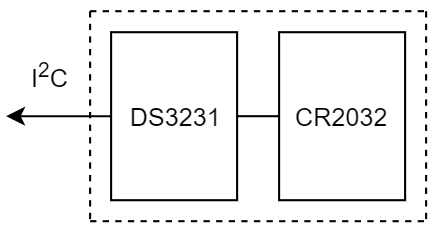
\includegraphics[scale=0.6]{graphics/Konzeptdiagramme/rtc.PNG}
	\caption{Real-Time-Clock (RTC)}
	\label{fig:rtc}
\end{figure}

